\documentclass[11pt]{article}
\usepackage[utf8]{inputenc}

\usepackage{amssymb, amsmath, amsthm, amsfonts, algorithmic, algorithm, graphicx}
\usepackage{color}
\usepackage{bbm}
\usepackage[dvipsnames]{xcolor} 
\usepackage[colorlinks,linkcolor=blue,citecolor=blue]{hyperref}
\usepackage{array}
\usepackage{ifthen}
\usepackage{subfigure}
\renewcommand{\baselinestretch}{1.1}
\setlength{\topmargin}{-3pc}
\setlength{\textheight}{8.5in}
\setlength{\oddsidemargin}{0pc}
\setlength{\evensidemargin}{0pc}
\setlength{\textwidth}{6.5in}

\newtheorem{theorem}{Theorem}[section]
\newtheorem{lemma}[theorem]{Lemma}
\newtheorem{proposition}[theorem]{Proposition}
\newtheorem{corollary}[theorem]{Corollary}
\newtheorem{question}[theorem]{Question}
\newtheorem{result}[theorem]{Result}
\newtheorem{definition}[theorem]{Definition}
\newtheorem{example}[theorem]{Example}
\newtheorem{remark}[theorem]{Remark}
\newtheorem{assumption}[theorem]{Assumption}
\numberwithin{equation}{section}

\def \endprf{\hfill {\vrule height6pt width6pt depth0pt}\medskip}
\renewenvironment{proof}{\noindent {\bf Proof} }{\endprf\par}

% Notational convenience,
% real numbers 
\newcommand{\R}{\mathbb{R}}  
% Expectation operator
\DeclareMathOperator*{\E}{\mathbb{E}}
% Probability operator
\DeclareMathOperator*{\Prob}{\mathbb{P}}
\renewcommand{\Pr}{\Prob}

% You may define additional macros here.


\begin{document}

\begin{center}
    \sc Recurrent and Generative ANNs
\end{center}

\noindent Name: Bileam Scheuvens, Pankaj Bora

\noindent Email: benedictbileam@gmx.de, bora.pankajt1@gmail.com

\noindent Matr. Nr.:6983475, 6946375



\section*{Exercise 1}
\subsection*{(a)}
See code for implementation.
\newline
After implementation of backprop, the given network quickly converges to a loss of less than 0.06 by around 350 epochs. It reduces further to less than 0.05 by the end of training with slight overfitting to the data. 


\begin{figure}[H]
  \centering
  \subfigure[Decision boundary at epoch 359]{
      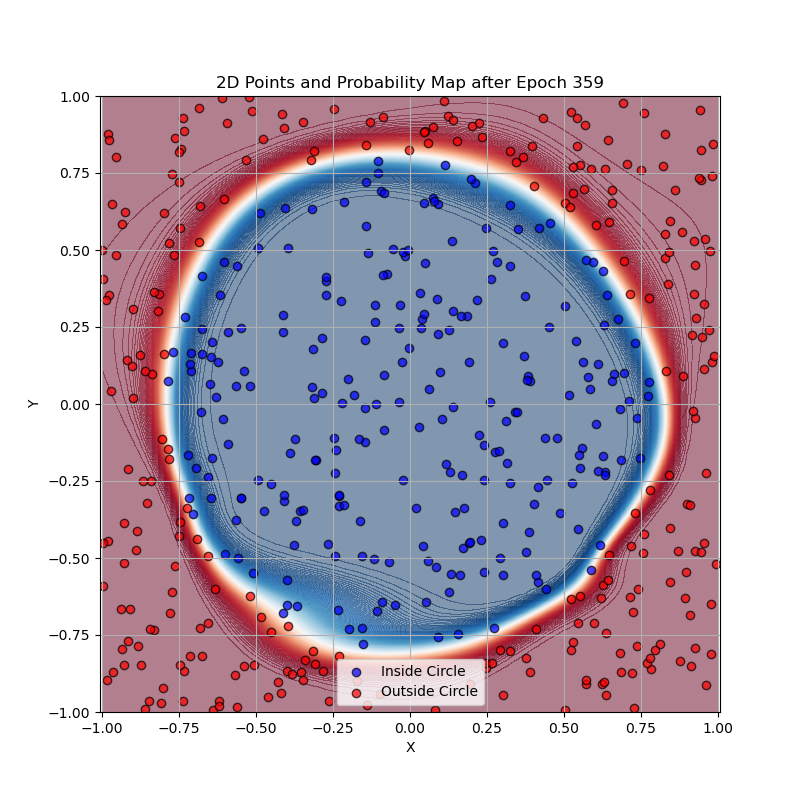
\includegraphics[width=0.45\textwidth]{images/e1_epoch350.png}
      \label{fig:epoch350}
  }
  \hspace{0.05\textwidth} % Adjust space between images
  \subfigure[Decision boundary at epoch 1024]{
      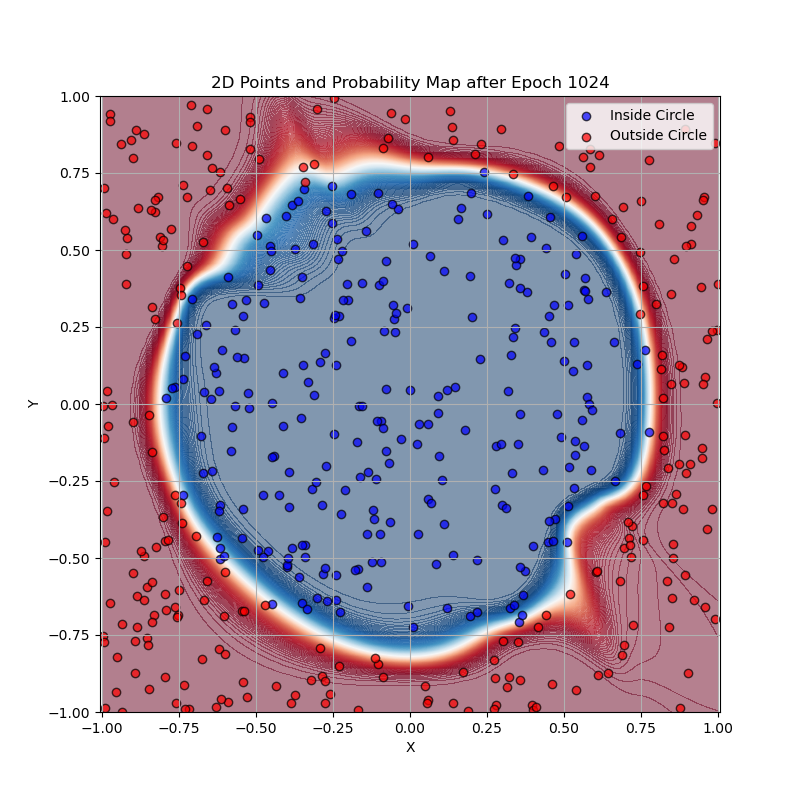
\includegraphics[width=0.45\textwidth]{images/e1_epoch1024.png}
      \label{fig:epoch1024}
  }
  \caption{Comparison of decision boundaries at different epochs}
  \label{fig:decision_boundaries}


\end{figure}

\begin{figure}[H]
  \centering % Centers the image
  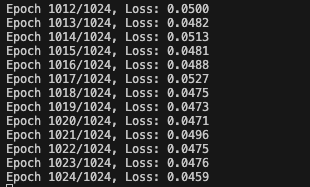
\includegraphics[width=0.5\textwidth]{images/e1_loss.png} % Adjust width as needed
  \caption{Loss values at the end} % Optional caption
\end{figure}

\subsection*{(b)}
\subsubsection*{1. Why is Cross-Entropy typically paired with the Softmax activation function?}
Softmax function, takes a vector of N real values and outputs a vector of N values that sum up to 1 (i.e a probability distribution). As cross entropy expects a probability distribution it is paired with the softmax activation function.

\subsubsection*{2. Gradient for CE with Softmax}

Given,
$softmax(z_j) = \frac{e^{z_j}}{\sum_k e^{z_k}}$
and
$L = - \sum_j y_j \log(softmax(z_j))$
\vspace{0.1cm}

$L = - \sum_j y_j \log\left(\frac{e^{z_j}}{\sum_k e^{z_k}}\right)$

$\quad= - \sum_j y_j \left( z_j - \log\left(\sum_k e^{z_k}\right) \right)$

$\quad= - \sum_j y_j z_j + \sum_j y_j \log\left(\sum_k e^{z_k}\right)$

\vspace{0.3cm}

$\frac{\partial}{\partial z_j} \left(- \sum_j y_j z_j\right) = -y_j$

\vspace{0.3cm}

$\frac{\partial}{\partial z_j} \left( \sum_j y_j \log\left(\sum_k e^{z_k}\right) \right) = \sum_j y_j \cdot \frac{1}{\sum_k e^{z_k}} \cdot e^{z_j} $
\vspace{0.3cm}

$\frac{\partial L}{\partial z_j} = \text{softmax}(z_j) \sum_j y_j - y_j$


\subsubsection*{3. Gradient for alternative normalization}

Given,
$\text{normalized}(z_j) = \frac{z_j}{\sum_k z_k}$
and 
$L = - \sum_j y_j \log\left(\frac{z_j}{\sum_k z_k}\right)$
\vspace{0.1cm}

$L = - \sum_j y_j \log(z_j) + \sum_j y_j \log\left(\sum_k z_k\right)$


$\frac{\partial}{\partial z_j} \left(- \sum_j y_j \log(z_j)\right) = -\frac{y_j}{z_j}$


$\frac{\partial}{\partial z_j} \left( \sum_j y_j \log\left(\sum_k z_k\right) \right) = \frac{\sum_j y_j}{\sum_k z_k}$


$\frac{\partial L}{\partial z_j} = \frac{\sum_j y_j}{\sum_k z_k} - \frac{y_j}{z_j}$

Comparing the gradients we can see that gradient with Softmax is much easier to simplify and compute. 

\section*{Exercise 2}
See code for implementation.

\section*{Exercise 3}

\begin{enumerate}
  \item{
\textbf{Network Configuration}
A hidden size of 3 leads to a hexagonal decision boundary.
The model thus has 3 layers, with 3 neurons each and a ReLU activation function after the first and second hidden layer.
}
\item{
\textbf{Theoretical Explanation}
Each ReLU is essentially a linear boundary.
Since the model has 6 neurons with ReLU and a hexagon is the best available approximation of a circle, it quickly finds this minimum.
  }

  \begin{figure}[H]
    \centering
    \subfigure[Decision boundary with 3 hidden layers]{
        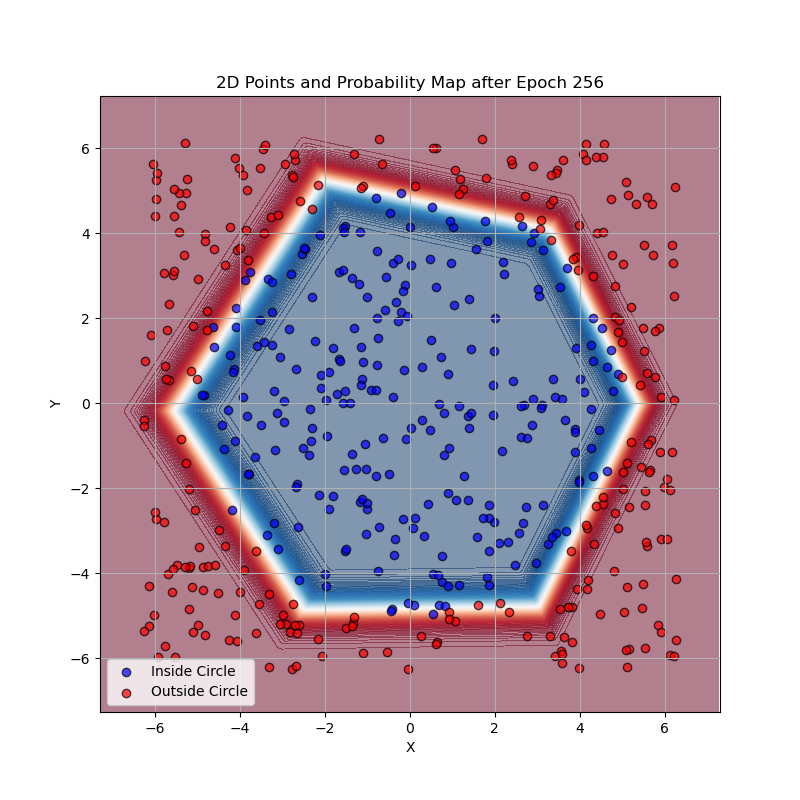
\includegraphics[width=0.45\textwidth]{images/Ex3_1.png}
        \label{fig:rh1}
    }
    \hspace{0.05\textwidth} % Adjust space between images
    \subfigure[Decision boundary with 3 hidden layers]{
        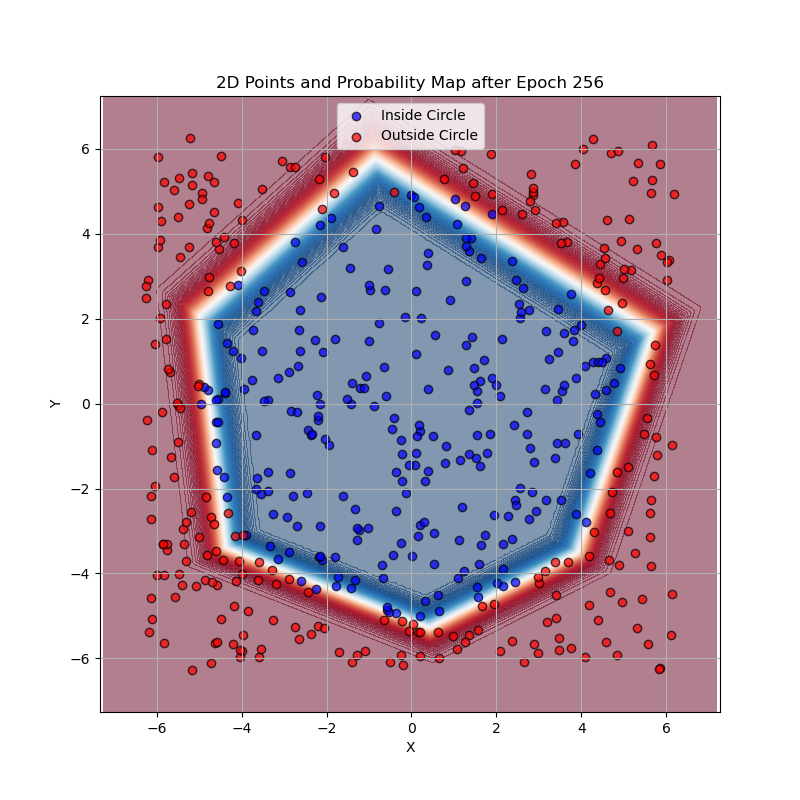
\includegraphics[width=0.45\textwidth]{images/Ex3_2.png}
        \label{fig:rh2}
    }
    \caption{Examples of output}
    \label{fig:rhrr}
  
  
  \end{figure}
\end{enumerate}
\end{document}
